\documentclass[11pt]{article}

\usepackage{../handout}
\usepackage{amsmath}
\usepackage{graphicx}

% Side margins:
% Actual margin is 1 in + this number
\oddsidemargin -0.25in
\evensidemargin -0.25in

% Text width:
\textwidth 6.9in

% Top margin:
% Actual margin is 1.5 in + this number
\topmargin -.3in

% Text height:
\textheight 8.7in


\begin{document}
\handout{12}{8}{Solutions to Written Assignment 3}

\begin{enumerate}

\item Consider the following class definitions.
\begin{verbatim}
class A {
  i : Int;
  o : Object;
  a : A <- new B;
  b : B <- new B;
  x : SELF_TYPE;
  f() : SELF_TYPE { x };
};
class B inherits A {
  g(b : Bool) : Object { (* EXPRESSION *) };
};
\end{verbatim}

Assume that the type checker implements the rules described in the
lectures and in the Cool Reference Manual.  For each of the following
expressions, occurring in place of \texttt{(* EXPRESSION *)} in the
body of the method \texttt{g}, show the static type inferred by the
type checker for the expression.  If the expression causes a type
error, give a brief explanation of why the appropriate type checking
rule for the expression cannot be applied.

\texttt{1)  i + i}

\texttt{Int}

\texttt{2)  x}

$\mathtt{SELF\_TYPE}_{\mathtt{B}}$

\texttt{3)  self = x}

\texttt{Bool}

\texttt{4)  self = i}

Error: \texttt{Int} objects can only be compared with other
\texttt{Int} objects

\texttt{5)  let x : B <- x in x}

\texttt{B}

\begin{verbatim}
6)  case o of
        o : Int => b;
        o : Bool => o;
        o : Object => true;
    esac
\end{verbatim}
\texttt{Bool}

\texttt{7)  a.f().g(b)}

Error: The class \texttt{A} does not have a method named \texttt{g}

\texttt{8)  f()}

$\mathtt{SELF\_TYPE}_{\mathtt{B}}$

\item Someone has proposed that Cool be extended to allow comparison,
addition, and multiplication operations on \texttt{Bool} objects as
well as on \texttt{Int} objects.  The comparison, addition, and
multiplication operations are now defined for any combination of
\texttt{Int} and \texttt{Bool} operands.  An addition or
multiplication operation involving an operand of type \texttt{Bool}
produces a result of type \texttt{Int} (the \texttt{Bool} object is
converted to $1$ if it has the value \texttt{true}, and to $0$ if it
has the value \texttt{false}).

Write the additional type checking rules (as in the lecture and the
Cool Reference Manual) for these operations on \texttt{Bool} objects.

The original type checking rule for arithmetic operations remains the
same for subtraction and division.

\begin{equation}
\begin{array}{c}
\begin{array}{l}
O, M, C \vdash e_{1} : Int \\
O, M, C \vdash e_{2} : Int \\
op \in \{-, /\}
\end{array} \\
\hline
O, M, C \vdash e_{1} \; op \; e_{2} : Int
\end{array}
\tag*{[Arith]}
\end{equation}

A new rule is added for addition and multiplication.

\begin{equation}
\begin{array}{c}
\begin{array}{l}
O, M, C \vdash e_{1} : T_{1} \\
O, M, C \vdash e_{2} : T_{2} \\
T_{1} \in \{Int, Bool\} \\
T_{2} \in \{Int, Bool\} \\
op \in \{*, +\}
\end{array} \\
\hline
O, M, C \vdash e_{1} \; op \; e_{2} : Int
\end{array}
\tag*{[Add-Mul]}
\end{equation}

The rule for non-equality comparisons must be extended to allow for
\texttt{Bool} operands.

\begin{equation}
\begin{array}{c}
\begin{array}{l}
O, M, C \vdash e_{1} : T_{1} \\
O, M, C \vdash e_{2} : T_{2} \\
T_{1} \in \{Int, Bool\} \\
T_{2} \in \{Int, Bool\} \\
op \in \{<, \leq\}
\end{array} \\
\hline
O, M, C \vdash e_{1} \; op \; e_{2} : Bool
\end{array}
\tag*{[Compare]}
\end{equation}

The rule for equality comparisons must be changed to allow for
comparisons between \texttt{Int} and \texttt{Bool} operands.

\begin{equation}
\begin{array}{c}
\begin{array}{l}
O, M, C \vdash e_{1} : T_{1} \\
O, M, C \vdash e_{2} : T_{2} \\
T_{1} = String \lor T_{2} = String \Rightarrow T_{1} = T_{2} \\
T_{1} \in \{Int, Bool\} \Rightarrow T_{2} \in \{Int, Bool\} \\
T_{2} \in \{Int, Bool\} \Rightarrow T_{1} \in \{Int, Bool\}
\end{array} \\
\hline
O, M, C \vdash e_{1} = e_{2} : Bool
\end{array}
\tag*{[Equal]}
\end{equation}

\item
\begin{enumerate}
\item Your friend Damon feels constrained by the fact that every
\texttt{while} expression in Cool evaluates to \texttt{void}.  He
would like to be able to write functions such as this:
\begin{verbatim}
f() : Bool {
  let x : Bool <- true in
    while x loop x <- false pool
};
\end{verbatim}
Damon wants to change the semantics of the \texttt{while} expression
so that the value of the expression is the value of the body on the
last execution of the loop.  He must define the value of a
\texttt{while} expression in the case that the body of the loop is
never evaluated, however.

Damon's first proposal is to define the value of the \texttt{while}
expression to be \texttt{void} when the predicate of the loop is
\texttt{false} initially and the body is never evaluated.  He says
that the type checker can now infer the static type of the
\texttt{while} expression to be the static type of the body, because
\texttt{void} is a member of every type.  Give an example Cool program
that shows how this change would cause a runtime type error (beyond
the existing Cool runtime errors), and explain how the error occurs.
\begin{verbatim}
class Main {
  main() : Int {
    5 + while false loop 7 pool
  };
};
\end{verbatim}

Under the proposed semantics, this program would be accepted by the
type checker because the type checker infers the static type
\texttt{Int} for the \texttt{while} expression.  At runtime, however,
the \texttt{while} expression evaluates to \texttt{void}, and so an
integer is added to \texttt{void}.  The result of this addition is
undefined, as under the standard definition of Cool an expression
whose static type is \texttt{Int} cannot take the value \texttt{void}
at runtime.  As such, a new runtime error is introduced into Cool.

\item After seeing your example, Damon comes up with a new suggestion.
He proposes to eliminate the requirement that the predicate expression
in a loop must be of static type \texttt{Bool}.  Now, the predicate
can have any static type, and a new method \texttt{is\_true() : Bool}
is added to the \texttt{Object} class.

The predicate is evaluated before each iteration of the loop.  If the
value of the predicate is \texttt{void}, the loop terminates.
Otherwise, the method \texttt{is\_true()} of the value of the
predicate is invoked, and the loop terminates if the value returned by
the method is \texttt{false}.  If the value returned by the method is
\texttt{true}, then the body of the loop is evaluated, and the process
repeats.  The value of the \texttt{while} expression is determined as
follows:

\begin{itemize}
\item If the body of the loop is never evaluated, then the value of
the \texttt{while} expression is the value of the predicate (from the
first evaluation of the predicate).

\item Otherwise, the value of the \texttt{while} expression is the
value of the body on the last execution of the loop.
\end{itemize}

Can these modified \texttt{while} semantics be type checked statically
to accept Damon's sample function above, while ensuring type safety
(i.e., that no runtime type error will occur)?  If so, write the most
flexible type rule (the rule that accepts the most correct programs)
for the modified \texttt{while} expression.  If not, explain why not,
and give an example Cool program that illustrates how this expression
can introduce new runtime errors (beyond the existing Cool runtime
errors).

\begin{equation}
\begin{array}{c}
\begin{array}{l}
O, M, C \vdash e_{1} : T_{1} \\
O, M, C \vdash e_{2} : T_{2} \\
\end{array} \\
\hline
O, M, C \vdash \text{while } e_{1} \text{ loop } e_{2} \text{ pool} :
T_{1} \sqcup T_{2}
\end{array}
\tag*{[Loop]}
\end{equation}

Under this type rule, the basic types \texttt{Int}, \texttt{String},
and \texttt{Bool} will be inferred by the type checker for a
\texttt{while} expression only if the type checker infers the same
basic type for both the predicate and the body of the loop.  The
existing rules of Cool do not allow an expression with static type
\texttt{Int}, \texttt{String}, or \texttt{Bool} to take the value
\texttt{void} at runtime.  As a result, a \texttt{while} expression
for which the type checker infers one of the static types
\texttt{Int}, \texttt{String}, or \texttt{Bool} will not evaluate to
\texttt{void}.  The only runtime errors caused by the \texttt{while}
expression are the runtime errors due to \texttt{void} that already
exist in Cool.

\item Damon wants to extend Cool by allowing method assignments.  He
would like to add a new assignment expression of the following form.
\begin{verbatim}
<exprB>.g <- <exprA>.f
\end{verbatim}
\noindent
Suppose that \texttt{<exprA>} evaluates to an object \texttt{a} of
class \texttt{A}, and \texttt{<exprB>} evaluates to an object
\texttt{b} of class \texttt{B}.  Furthermore, \texttt{A} has a method
named \texttt{f} and \texttt{B} has a method named \texttt{g}, and
the two methods \texttt{f} and \texttt{g} have the same signature (the
signature consists of the number of arguments, the types of the formal
parameters, and the return type).  The effect of the assignment would
be to set the body of the method \texttt{g} of the object \texttt{b}
to the body of the method \texttt{f} of the object \texttt{a}, so that
subsequent invocations of the method \texttt{g} belonging to
\texttt{b} would execute the body of the method \texttt{f} belonging
to \texttt{a}.  The value of the assignment expression would be
\texttt{void}.

Damon says that, if \texttt{B} is a subclass of \texttt{A} (a
descendant of \texttt{A} in the inheritance graph), then the
inheritance rules of Cool guarantee that this operation is type safe.

Can Damon's method assignment expression be type checked statically to
guarantee type safety?  If so, write the most flexible type rule for
the method assignment expression.  If not, explain why not, and give
an example Cool program that illustrates how this expression can
introduce new runtime errors (beyond the existing Cool runtime
errors).

This method assignment expression cannot be type checked statically
while ensuring type safety because the dynamic types of the objects
involved in the assignment may be different from the static types.
The type checker cannot guarantee at compile time that the dynamic
type of the object to which the method is being assigned is a subclass
of the dynamic type of the object that contains the method being
assigned.
\begin{verbatim}
class A {
  x : Int;
  f(z : Int) : Int {
    z + x
  };
};
class B inherits A {
  y : Int;
  f(z : Int) : Int {
    z + x + y
  };
};
class Main {
  main() : Object {
    let a : A <- new A,
        b : A <- new B in {
      a.f <- b.f;
      a.f(1);
    }
  };
};
\end{verbatim}

Any static type rule for the method assignment expression would have
to allow the method assignment \texttt{a.f <- b.f} in this program,
because the static types of \texttt{a} and \texttt{b} are the same.
However, executing this program would lead to a runtime error because
the object \texttt{a} does not have an attribute \texttt{y}.
\end{enumerate}

\item Suppose \texttt{f} is a function with a call to \texttt{g}
somewhere in the body of \texttt{f}.
\begin{verbatim}
f(...) {
 ... g(...) ...
}
\end{verbatim}
We say that this particular call to \texttt{g} is a {\it tail call}
if the call is the last thing \texttt{f} does before returning.  For
example, consider the following two functions for computing positive
powers of $2$.
\begin{verbatim}
f(x : Int, acc : Int) : Int { if (0 < x) then f(x - 1, acc * 2) else acc fi };
g(x : Int) : Int { if (0 < x) then (2 * g(x - 1)) else 1 fi };
\end{verbatim}
Here $\verb'f(x, 1)' = \verb'g(x)' = 2^x$ for $x\geq 0$.  The
recursive call to \texttt{f} is a tail call, while the recursive call
to \texttt{g} is not.  A function in which all recursive calls are
tail calls is called {\it tail recursive}.

\begin{enumerate}
\item Here is a non-tail recursive function for computing factorials.
\begin{verbatim}
fact(n : Int) : Int { if (0 < n) then (n * fact(n - 1)) else 1 fi };
\end{verbatim}
Write a tail recursive function \texttt{fact2} that computes the same
result.  (Hint: Your function will most likely need two arguments, or
it may need to invoke a function of two arguments.)
\begin{verbatim}
fact2(n : Int, acc : Int) : Int {
  if (n = 0)
  then acc
  else fact2(n - 1, acc * n)
  fi
};
\end{verbatim}

\item Recall from lecture that function calls are usually implemented
using a stack of activation records.  Trace through the execution of
\texttt{fact} and \texttt{fact2} as they compute $4!$, showing the
tree of activation records (each node of the tree shows the invocation
of a function, and the arguments).  How can a compiler make the
execution of the tail recursive function \texttt{fact2} more efficient
than that of \texttt{fact}?  (Hint: Compare the stack space required
for \texttt{fact(99)} with the stack space required for
\texttt{fact2(99)}.  Can \texttt{fact2} use fewer activation records?)

The function invocations, with arguments, are as follows.
\begin{align*}
& \mathtt{fact(4)} \rightarrow \mathtt{fact(3)} \rightarrow
\mathtt{fact(2)} \rightarrow \mathtt{fact(1)} \rightarrow
\mathtt{fact(0)} \\
& \mathtt{fact2(4, 1)} \rightarrow \mathtt{fact2(3, 4)} \rightarrow
\mathtt{fact2(2, 12)} \rightarrow \mathtt{fact2(1, 24)} \rightarrow
\mathtt{fact2(0, 24)}
\end{align*}

A compiler can compile a tail recursive function such as
\texttt{fact2} so that a new activation record is not needed for every
recursive invocation of \texttt{fact2} in a computation.  Suppose that
the method \texttt{fact2} is invoked with the arguments $4$ and $1$
from a function \texttt{main}.  The return address in the activation
record for this invocation is an address $R$ that specifies an
instruction in the body of \texttt{main}.

Since \texttt{fact2} is tail recursive, after the recursive invocation
of \texttt{fact2} with the arguments $3$ and $4$ has completed, no
further computation must be done in the body of \texttt{fact2} to
complete the invocation \texttt{fact2(4, 1)}.  The return value of
\texttt{fact2(3, 4)} is the return value of \texttt{fact2(4, 1)}.  As
a result, the compiler can replace the activation record for
\texttt{fact2(4, 1)} with the activation record for
\texttt{fact2(3, 4)}.  The return address for \texttt{fact2(3, 4)} is
the same as the return address for \texttt{fact2(4, 1)} ($R$), and the
return value of \texttt{fact2(4, 1)} is now set during the execution
of \texttt{fact2(3, 4)}.  Figure \ref{artail} illustrates the stack
space saved by this compiler optimization, showing the activation
records during the invocation \texttt{fact2(3, 4)}.
\begin{figure}[htb]
\begin{center}
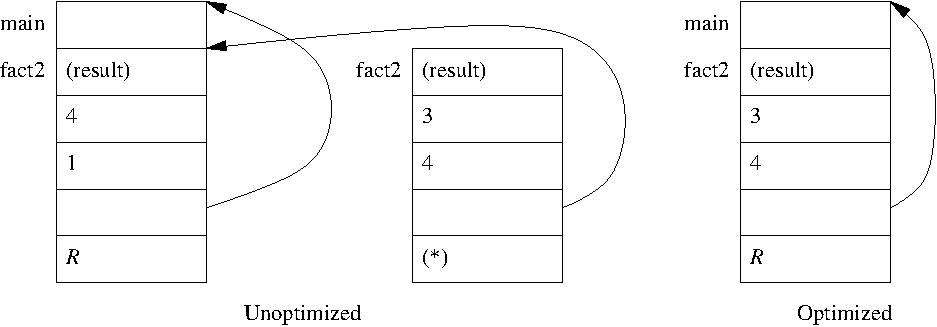
\includegraphics{artail}
\caption{Activation records during the function invocation
\texttt{fact2(3, 4)}.}
\label{artail}
\end{center}
\end{figure}
\end{enumerate}

\item In some languages, a class can have multiple methods with the
same name, as long as these methods differ in the number and/or types
of formal parameters.  This is referred to as method
{\em overloading}.

Suppose we would like to add method overloading to Cool.  Now, when
generating code for a dispatch expression
$e_{0}.f(e_{1}, \dots, e_{n})$, the compiler may need to choose the
method to dispatch to (i.e., which slot in the dispatch table to jump
to) amongst several valid possibilities.  Let $T_{i}$ be the static
type of $e_{i}$ for $i = 0, 1, \dots, n$.  Suppose that the compiler
chooses a method $f$ for the dispatch such that:
\begin{itemize}
\item $T_{0}$ has a method $f$ with $n$ formal parameters of types
$P_{1}, \dots, P_{n}$; and

\item $T_{i} \leq P_{i}$ for $i = 1, \dots, n$; and

\item If $T_{0}$ has more than one method named $f$, then, for any
other method named $f$ with $n$ formal parameters
$Q_{1}, \dots, Q_{n}$ satisfying $T_{i} \leq Q_{i}$ for
$i = 1, \dots, n$, it must be the case that $P_{i} \leq Q_{i}$ for
$i = 1, \dots, n$.  In other words, $P_{1}, \dots, P_{n}$ are the most
specific parameter types for a method named $f$ that could be invoked.
\end{itemize}

If a {\em unique} method exists under these rules, then the dispatch
is accepted by the type checker.  If more than one method satisfies
these conditions, then the type checker signals a type error at
compile time.

Method overriding occurs as described in the original Cool Reference
Manual.  Specifically, a method defined in a child class overrides any
method with the identical signature in the parent class.

Consider the following Cool program:
\begin{verbatim}
class A inherits IO {
  f(a : Object, b : Object) : Object { out_string("1") };   (* offset 0 *)
  f(a : Object, b : Int) : Object { out_string("2") };      (* offset 1 *)
};
class B inherits A {
  f(a : Object, b : Object) : Object { out_string("3") };   (* offset 0 *)
  f(a : Int, b : Object) : Object { out_string("4") };      (* offset 2 *)
};
class Main {
  main() : Object {
    let a : A <- new B,
        b : B <- new B,
        x : Object <- new Object,
        y : Object <- 1,
        z : Int <- 2 in
      (* DISPATCH *)
  };
};
\end{verbatim}

For each of the following dispatch expressions, give the output of the
program when \texttt{(* DISPATCH *)} is replaced by the dispatch
expression, or specify that a type error would occur.

The compiler chooses an offset in the dispatch table for a method
invocation at compile time, based on the static types of the
arguments.  When the invocation occurs at runtime, the method that
executes is the method at that offset in the dispatch table.  The
following table shows the method offset chosen by the compiler
(assuming the offsets are fixed according to the numbers in the
comments in the program) and the output for each of the dispatch
expressions.
\begin{center}
\begin{tabular*}{0.5\textwidth}{@{\extracolsep{\fill}}lcc}
Dispatch & Offset & Output \\
\hline
\texttt{a.f(x, x)} & 0 & \texttt{3} \\
\texttt{a.f(x, y)} & 0 & \texttt{3} \\
\texttt{a.f(x, z)} & 1 & \texttt{2} \\
\texttt{a.f(y, x)} & 0 & \texttt{3} \\
\texttt{a.f(y, y)} & 0 & \texttt{3} \\
\texttt{a.f(y, z)} & 1 & \texttt{2} \\
\texttt{a.f(z, x)} & 0 & \texttt{3} \\
\texttt{a.f(z, y)} & 0 & \texttt{3} \\
\texttt{a.f(z, z)} & 1 & \texttt{2} \\
\texttt{b.f(x, x)} & 0 & \texttt{3} \\
\texttt{b.f(x, y)} & 0 & \texttt{3} \\
\texttt{b.f(x, z)} & 1 & \texttt{2} \\
\texttt{b.f(y, x)} & 0 & \texttt{3} \\
\texttt{b.f(y, y)} & 0 & \texttt{3} \\
\texttt{b.f(y, z)} & 1 & \texttt{2} \\
\texttt{b.f(z, x)} & 2 & \texttt{4} \\
\texttt{b.f(z, y)} & 2 & \texttt{4} \\
\texttt{b.f(z, z)} & 1 or 2 & TYPE ERROR
\end{tabular*}
\end{center}

\end{enumerate}

\end{document}
